\onecolumn
\section{Proof of Proposition~\ref{prop:mde}}
\label{sec:proof}
\begin{proof}
Standard analysis of maximum likelihood estimation suggests that whenever the class of distributions $\cP$ that $p$ is chosen from is expressive enough, then the optimal solution $p^\star_\lambda = \arg\min_{p\in\cP} L_\lambda(p)$ satisfies: 
\begin{equation}
    \E_{x\sim D_x} \|p^\star_\lambda(\cdot | x) - \sum_i \lambda_i D_{i,y}(\cdot | x)\|_1 \leq \epsilon,
    \label{eq:tv-bound}
\end{equation}

where $\epsilon$ is a parameter which depends on the sample size $n$ and the statistical complexity of the function class $\cP$~\citep{geer2000empirical, zhang2006varepsilon}. For example, the statistical complexity is equal to $\ln|\cP|$ for finite classes, and can be replaced with a log-covering number more generally. The main takeaway from Equation~\ref{eq:tv-bound} is that the optimal solution $p^\star_\lambda$ can be written as $p^\star_\lambda = \sum_i \lambda_i p^\star_{e_i}$ in this case, where $e_i$ is the $i_{th}$ basis vector with all zeros and one in the $i_{th}$ position.

More generally, when the marginal distributions over $x$ are different, we can write 
\begin{align*}
    p^\star_{\lambda}(y|x) =& \sum_i p(i | x) D_i(y|x) = \sum_i \frac{p(x|i)p(i)}{\sum_j p(x|j)p(j)} D_i(y|x)\\ 
    =& \sum_i \frac{D_i(x)\lambda_i}{\sum_j \lambda_j D_j (x)} D_i(y|x)\\ =& \sum_i \lambda_i^{'} p^\star_{e_i},
\end{align*}
%
\end{proof}




\section{Implementation Details}
\label{sec:appendix_implementation}






\subsection{Model and training details}
\label{sec:appendix_lms}
Table \ref{model-sizes} specifies the model sizes used during the experiments. Note that, due to the large vocabulary size, the number of non-embedding parameters is much smaller than the number of total parameters. For example, our $280$M proxy models have fewer non-embedding parameters than \textsc{DoGe-124M}.

Models of all sizes used batch size of $512$ sequences of up to $1024$ text tokens. The maximum number of steps $200$K corresponds to about $100$B tokens. All language models were optimized using Adafactor~\cite{adafactor} with initial learning rate of 1e-3, weight decay of 1e-2, and gradient clipping to norm 1. We decay the learning rate exponentially until it reaches a minimum of 1e-4 at the end of training, with a linear
warmup of 6\% of the total training steps.

Table ~\ref{hardware} details the Google Cloud TPU configurations used to train models of each size.
%The $70$M models take about $1.2$ hours to train to 10K steps (5B tokens) and the computational requirements scale approximately linearly with model size. The final models used for regression and mixture optimization were 25 models of size $280$M trained for 10K steps.

%\lc{Should we also include the number of train tokens?}

\begin{table}[htbp]
\begin{center}
\begin{small}
\begin{sc}
\scalebox{1.0}{
\begin{tabular}{rrrrrr}
\toprule
Model size & Model dim. & \# Layers & Hidden dim. & \# Attention heads & Non-embedding params \\
\midrule
70M & $256$  & $3$ & $1{,}024$ & $4$ & $2{,}625{,}984$ \\
150M & $512$ & $6$ & $2{,}048$ & $8$ & $19{,}171{,}712$ \\
280M & $768$ & $12$ & $3{,}072$ & $12$ & $85{,}312{,}768$ \\
510M & $1{,}024$ & $12$ & $8{,}192$ & $16$ & $252{,}125{,}952$ \\
1B & $2{,}048$ & $16$ & $8{,}192$ & $32$ & $805{,}993{,}472$ \\
\bottomrule
\end{tabular}
}
\end{sc}
\end{small}
\end{center}
\caption{Architecture details for models used in our experiments. All models use the same vocabulary with a size of $256{,}000$.}
\label{model-sizes}
\end{table}



\begin{table}[htbp]
\begin{center}
\begin{small}
\begin{sc}
\scalebox{1.0}{
\begin{tabular}{rr}
\toprule
Model size &   TPU v3 chips\\
\midrule
70M &  $16$ \\
150M &  $16$ \\ 
280M & $32$ \\
510M & $32$ \\
1B & $64$ \\
\bottomrule
\end{tabular}
}
\end{sc}
\end{small}
\end{center}
\caption{Hardware used for each model size.}
\label{hardware}
\end{table}




\subsection{Expert mixtures as regression examples}

When fitting regression model with MDE features we experimented with both using the expert mixtures as examples and not using them, as expert mixtures like $(1,0,0, ...)$ may exhibit significantly different behavior from near-corner mixtures such as $(1-\epsilon, \epsilon, 0, ...)$. We evaluated whether including these corner mixtures enhances or degrades model generalization performance. For Linear-MDE and GBM-MDE, we found that adding expert mixtures degrades performance, whereas for MTGP-MDE, it improves performance. We speculate that MTGP offers greater flexibility in modeling behavior at the corners without compromising predictions at other points. Nonetheless, when reporting the number of training examples, we always account for the expert examples used to generate the MDE features, ensuring that expert mixtures are included in the training example count.

\subsection{Generating training mixture examples}
\label{sec:generating_training_mixture_examples}
Our goal is to sample a diverse set of mixture examples to fit a regression model that generalizes well across the entire mixture search space while also accounting for training domain token frequency. \cite{regmix} suggested sampling from a Dirichlet distribution and setting the concentration parameters based on token frequency of the training domains. We opted to  emphasize less prior domain token counts, as lower value training domains may contain a higher number of tokens. Instead, we set the concentration parameters as a weighted average between domain frequency and a uniform distribution. Additionally, we sampled scaling factors between 0.5 and 2.0 and multiplied the concentration parameters with them to introduce varying levels of diversity. 
%We used mixtures sampled with the same approach and mixtures from prior work for evaluation.


\subsection{Splitting Examples for Training and Testing}
To assess model performance, we randomly split the mixture examples into training and test sets five times. For each metric, we computed the sample mean and 95\% confidence interval, and verified results we highlighted as different did not have overlapping confidence intervals. The reported loss-related squared error and ranking metrics represent the mean across the five folds.

\subsection{Fitting Regression Models}
\label{ref:appendix_fitting_regression_models}

\noindent \textbf{MTGP} - We trained the multi-task Gaussian process with a separable kernel using the open-source Vizier framework \cite{vizier}.  

\noindent \textbf{Gradient Boosting} - We initially considered using the default LightGBM \cite{lightgbm} setup from \cite{regmix}. However, its default minimum leaf size is 20, which is unsuitable to our low-data regime of about 20 examples. Instead, we used Scikit-Learn's \cite{scikit-learn} gradient boosting model and performed a 5-fold cross-validation hyper-parameter grid search over the number of estimators \(\{10, 50, 100\}\), learning rate \(\{0.01, 0.1\}\), and maximum tree depth \(\{2, 3, 4\}\). For the rest of the  hyper-parameters we used the default settings.

\noindent \textbf{Linear} - We trained a Scikit-Learn linear model with Ridge regularization and performed 5-fold cross-validation to tune the regularization factor.

\subsection{Additional dataset details}
\label{sec:appendix_data}

%\textcolor{red}{Add validation and test set sizes and license information. Confirm we are using the data in a way consistent with the licenses.}


All training and evaluation datasets are predominantly in English, with possible exceptions for some SlimPajama texts.


We list the number of tokens in each of the 18 validation domains we used for loss optimization in Table ~\ref{tab:validation_domains}. For the end-task derived datasets, both the question and gold response are included in the token counts.


\begin{table}[htbp]
\begin{center}
\begin{small}
\begin{sc}
\scalebox{1.0}{
\begin{tabular}{lr}
\toprule
Domain &   Number of Tokens\\
\midrule
ArXiv & 4,105,850 \\
Book & 4,188,414 \\
C4 & 1,719,076 \\
CommonCrawl & 3,281,676 \\
Github & 2,861,175\\
StackExchange & 2,265,251\\
Wikipedia & 2,131,781 \\
\midrule
ARC-c-0shot & 43,413 \\
ARC-c-1shot & 87,117\\
ARC-c-5shot & 258,026\\

ARC-e-0shot & 74,902\\
ARC-e-1shot & 152,276 \\
ARC-e-5shot & 455,940 \\
MultiRC-0shot & 2,704,800 \\
MultiRC-1shot & 3,581,458 \\
OpenBookQA-0shot & 12,743 \\
OpenBookQA-1shot & 26,175 \\
OpenBookQA-5shot & 82,318 \\
\bottomrule
\end{tabular}
}
\end{sc}
\end{small}
\end{center}
\caption{Number of tokens in validation domains used for loss prediction and optimization.}
\label{tab:validation_domains}
\end{table}


\subsection{Use of AI Assistants}

We have used Gemini models to understand tikz for drawings and to suggest ways to format equations and algorithms. We also used Gemini to suggest ways to shorten some sentences and took some suggestions with additional edits.


\section{Additional results and analysis}

\label{sec:appendix_results}


\subsection{Comparing Optimized Mixtures Across Different Scales}

To better understand the impact of model size and training steps on the optimized mixture, we compare the mixtures obtained using the \textsc{LINEAR+MDE} method for two different models: (i) 70M-parameter model trained for 10K steps, and (ii) 280M-parameter model trained for 50K steps.

\vspace{0.5em} % Adds a small vertical space

\noindent
The optimized mixture for the \textit{70M, 10K-step} model is:  
\[
[0.078, 0.28, 0.411, 0.072, 0.0, 0.012, 0.148]
\]
The optimized mixture for the \textit{280M, 50K-step} model is:
\[
[0.039, 0.287, 0.373, 0.259, 0.0, 0.0, 0.041]
\]

\noindent
Despite differences in model scale and token horizon, the mixture weights remain relatively similar, with a \textbf{cosine similarity of 91.32\%}. This strong alignment further supports the validity of our proxy model mixture optimization approach.

\subsection{Correlation among losses of different validation domains}

\begin{figure*}[htbp]
\vskip 0.2in
\begin{center}
\scalebox{0.7}{
\centerline{\includegraphics[width=\columnwidth]{figures/loss_correlation.png}}
}
\caption{Correlation among model losses on different heldout training and end task domain datasets.}
\label{fig:validation_loss_correlation}
\end{center}
\vskip -0.2in
\end{figure*}


From Figure~\ref{fig:validation_loss_correlation} we see that the SlimpPajama domains most correlated with validation end task domains are Book, C4, and CommonCrawl.

%The MDE models are optimized from 7 models of size 280M at 10K steps (checked colab Feb 8)
\subsection{Mixture rates for SlimPajama from baselines and our work}

In the experiments section, we reported losses and downstream from baseline mixtures, ones derived in prior work (in which case we copied the mixture rate values from the respective papers), and mixtures optimized in this work. Here we list the mixture proportion values $\lambda$ for completeness in Tables ~\ref{mixture-weights-prior} and ~\ref{mixture-weights-this-work}.

\begin{table}[htbp]
\begin{center}
\begin{small}
\begin{sc}
\scalebox{0.8}{
\begin{tabular}{lrrrrr}
% 6 columns
\toprule
Domain & Uniform & SlimPajama & DoGE-124M & DoReMi-124M & DML \\
\midrule
Arxiv  &  0.1429 &  0.0458 &   0.0890 &   0.0434 &   0.2500 \\
Book  &  0.1429 &   0.0420 &  0.0456 &  0.0546 &  0.0938 \\
C4  &  0.1429 &  0.2660 &   0.2789 &  0.1127 & 0.2500  \\
CommonCrawl  &  0.1429 & 0.5203 & 0.1968 & 0.3781 & 0.1250 \\
Github  &  0.1429 & 0.0522 & 0.0714 & 0.0753 & 0.1406  \\
StackExchange  &  0.1429 & 0.0337 & 0.1703 & 0.0919 & 0.1250\\
Wikipedia  &  0.1429 & 0.0399 & 0.1480 & 0.2440 & 0.0156  \\
\bottomrule
\end{tabular}
}
\end{sc}
\end{small}
\end{center}
\caption{SlimPajama data mixture rates derived through different approaches from prior work. DoGE and DoReMI weights are from the SlimPajama experiments of ~\cite{DOGE}. DML weights are copied from ~\cite{dml}.} % results are at 200K steps
\label{mixture-weights-prior}
\end{table}



\begin{table}[htbp]
\begin{center}
\begin{small}
\begin{sc}
\scalebox{0.8}{
\begin{tabular}{lrrrrrr}
\toprule
Domain & \textsc{MTGP-mde-sp} & \textsc{Linear-mde-et} & \textsc{Linear-mde-all} & \textsc{MDE-sp} & \textsc{MDE-et} & \textsc{MDE-all} \\
\midrule
Arxiv  &  0.0791 & 0.0014 & 0.0404 & 0.0666 & 0.0015 & 0.0372 \\
Book  &  0.0931 & 0.2412 & 0.2859 & 0.1870 & 0.3251 & 0.2732 \\
C4  &  0.2282 & 0.2952 & 0.3710 & 0.0837 & 0.3286 & 0.1868 \\
CommonCrawl  &  0.1335 & 0.4578 & 0.2581 & 0.1602 & 0.2734 & 0.2249 \\
Github  &  0.1047 & 0.0014 & 0.0014 & 0.1161 & 0.0000 & 0.0395 \\
StackExchange  &  0.1454 & 0.0014 & 0.0014 & 0.2187 & 0.0715 & 0.1575 \\
Wikipedia  &  0.2161 & 0.0014 & 0.0418 & 0.1678 & 0.0000 & 0.0810 \\
\bottomrule
\end{tabular}
}
\end{sc}
\end{small}
\end{center}
\caption{SlimPajama data mixture rates derived through optimizing \textsc{avg-sp}, \textsc{avg-et}, and \textsc{avg-sp}+\textsc{avg-et} with regressors using MDE or MDE on its own.} % results are at 200K steps
\label{mixture-weights-this-work}
\end{table}


\subsection{Loss learning curve for 1B models}

Figure~\ref{fig:convergence_curve} shows the average \textsc{sp} domain loss of 1B models with different data mixture proportions. We see that MTGP-MDE-SP achieves lower loss than other approaches.

\begin{figure}[htbp] % Ensure proper floating behavior
  \centering
  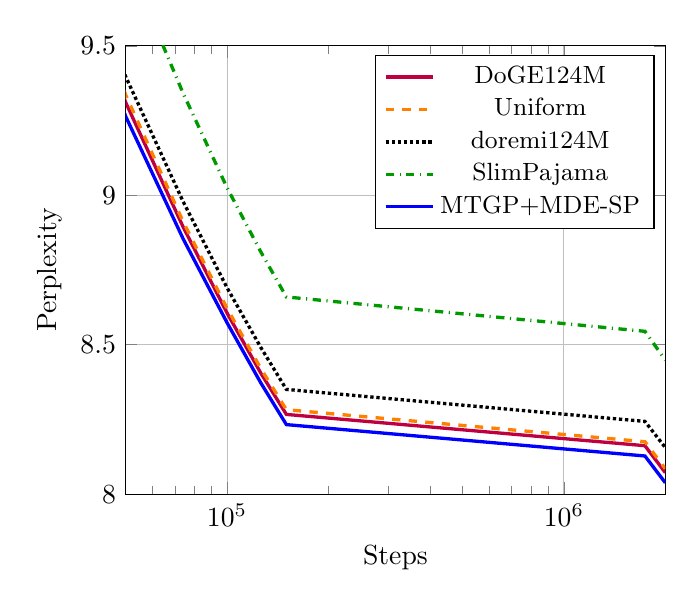
\begin{tikzpicture}
    \begin{axis}[
      xlabel={Steps},
      ylabel={Perplexity},
      legend pos=north east, % Keep legend at the top right
      grid=major,
      xmin=50000, xmax=2000000,
      ymin=8, ymax=9.5,
      xmode=log, % Logarithmic x-axis
      log basis x=10,
      every axis plot post/.append style={
          very thick
      },
      legend style={
          draw=black, % Adds a border around the legend
          at={(0.98,0.98)}, anchor=north east, % Fine-tuned legend placement
          font=\small, % Adjust font size if needed
          fill=white, % Keeps legend background white
          /tikz/every even column/.append style={column sep=0.5cm}
      }
    ]
      % DoGE124M
      \addplot[purple, very thick] coordinates {
        (10000, 12.1210) (20000, 10.5785) (50000, 9.3106) 
        (74000, 8.8948) (100000, 8.6058) (126000, 8.4046) 
        (150000, 8.2667) (1740000, 8.1620) (2000000, 8.0719)
      };
      \addlegendentry{DoGE124M}
      
      % Uniform (Changed to dashed)
      \addplot[orange, dashed, very thick] coordinates {
        (10000, 12.1843) (20000, 10.6228) (50000, 9.3356) 
        (74000, 8.9126) (100000, 8.6213) (126000, 8.4200) 
        (150000, 8.2825) (1740000, 8.1753) (2000000, 8.0849)
      };
      \addlegendentry{Uniform}
      
      % doremi124M
      \addplot[black, densely dotted, very thick] coordinates {
        (10000, 12.2241) (20000, 10.6653) (50000, 9.3972) 
        (74000, 8.9797) (100000, 8.6903) (126000, 8.4904) 
        (150000, 8.3504) (1740000, 8.2433) (2000000, 8.1558)
      };
      \addlegendentry{doremi124M}
      
      % SlimPajama
      \addplot[green!60!black, dashdotted, very thick] coordinates {
        (10000, 12.9377) (20000, 11.2072) (50000, 9.7975) 
        (74000, 9.3421) (100000, 9.0251) (126000, 8.8102) 
        (150000, 8.6597) (1740000, 8.5447) (2000000, 8.4486)
      };
      \addlegendentry{SlimPajama}
      
      % MTGP+MDE-SP
      \addplot[blue, very thick] coordinates {
        (10000, 12.0681) (20000, 10.5314) (50000, 9.2640) 
        (74000, 8.8551) (100000, 8.5734) (126000, 8.3718) 
        (150000, 8.2326) (1740000, 8.1276) (2000000, 8.0380)
      };
      \addlegendentry{MTGP+MDE-SP}

    \end{axis}
  \end{tikzpicture}
  \caption{Convergence curve of training 1B parameter model for up to 200K steps for the different methods.}
  \label{fig:convergence_curve}
\end{figure}




\subsection{Optimizing mixtures with MDE only}
%\todo{Add details}
We additionally optimize the mixtures for different criteria using the MDE approximation only, from 280M-sized models at 6K training steps. This requires training only seven proxy language models and no regression. In Table~\ref{loss-1b-withendtask-mde}, we see that models optimized for \textsc{avg-sp} based on MDE lead to worse but respectable \textsc{avg-sp} loss than MTGP-\textsc{mde}. Models optimized for the end task validation domains are best on those domains, and models optimized for average of SlimPajama and ET domains achieve slightly better tradeoff between those groups of domains than models optimized for ET domains only.


\begin{table}[htbp]
\begin{center}
\begin{small}
 \begin{sc}
 \scalebox{0.8}{
 \begin{tabular}{lrrrrrr}
 \toprule
 Domain &  \textsc{MTGP-mde-sp}  & \textsc{Linear-mde-et} & \textsc{Linear-mde-all} & \textsc{MDE-sp} & \textsc{MDE-et} & \textsc{MDE-all} \\
 \midrule
 Avg. SP  & \textbf{8.04} & 10.44  & 9.26 & 8.110 & 10.501 & 8.228 \\
 Avg. task  &  22.89 & \textbf{19.96} & 20.59 & 23.246 & {20.439} & 21.800 \\
 \bottomrule
 \end{tabular}
 }
 \end{sc}
 \end{small}
 \end{center}
 \caption{Generalization on SlimPajama and end task validation domains for 1B models trained for 100B tokens. Comparing MDE to MTGP-\textsc{mde} and \textsc{Linear-mde} optimized weights. We report average perplexities on SlimPajama and end task validation domains.} 
 \label{loss-1b-withendtask-mde}
 \end{table}
 

 
 
 \subsection{MDE vs relatated approximations through domain-specific expert models}
 
 \label{sec:model_merge}
 

 To understand the performance of MDE in the context of related ideas from ~\citet{emnlp-merge}, which, as mentioned in Section~\ref{sec:related}, approximates the loss of a model trained on a union of datasets with the loss of a model which is a parameter average of expert models trained on the individual datasets, we analyze the importance of using model ensembles instead of parameter-averaged models. In addition, we evaluate MDE in comparison to a simpler and even faster to compute version, which interpolates per-dataset average probabilities instead of per-token ones.


We compute Spearman's rank correlation between the true domain losses
versus the ones predicted by MDE and the two alternative methods, using 20 models of size 280M trained for 10K steps, corresponding to 20 different data mixtures. We report $\rho$ across the seven SplimPajama domains, and also average across the full 18 domains (SlimPajama and end-task validation domains).  Table~\ref{mde-merge-interpolate} shows the results. Note that these metrics are averages of performance for predicting single domain losses, and are a bit higher than the metrics for predicting aggregated losses that we saw in Table~\ref{tab:regressors_sxs}. We can note that model merging, where for each candidate $\lambda$ we first compute a weighted average of expert model parameters, and then run inference to compute losses on the validation domains, has very poor performance. This agrees with prior work which finds parameter averaging to work well only for models fine-tuned from a common initialization points.  The per-domain interpolation approach does not use token-level probabilities from the experts, but only computes a weighted average (with $\lambda$) of their per-validation dataset average probabilities. We see that this approach does surprisingly well, but is still substantially weaker than MDE. 

Based on these results we conclude that parameter averaging of expert models  is not a useful approach for approximating losses for pre-training data mixtures. We also see that there is value in interpolating per-token probabilities, as in MDE, instead of interpolating per-dataset average probabilities. Per-dataset probability interrelation is a bit easier to implement and faster to compute, and could also be useful. Future work could also explore both MDE and per-domain interpolation as feature sources in the same regression model.



\begin{table}[htbp]

\vskip 0.15in
\begin{center}
\begin{small}
\begin{sc}
\scalebox{0.8}{
\begin{tabular}{lrrr}
\toprule
  & MDE  & Model Merging  & Per-Domain \\ 
  &  &  & Interpolation \\
\midrule
\textsc{SP} Spearman & \textbf{0.951} & -0.139 & 0.898 \\
\textsc{All} Spearman &  \textbf{0.942} & -0.120 & 0.927 \\

\bottomrule
\end{tabular}
}
\end{sc}
\end{small}
\end{center}
\vskip -0.1in
\caption{MDE versus Model Merging and Per-Dataset Interpolation.} % results are at 200K steps
\label{mde-merge-interpolate}
\end{table}









